\chapter{Enfoque bayesiano}

En esta sección complementaremos el enfoque visto hasta ahora en cuanto a la incorporación de un modelo para la incertidumbre asociada al parámetro $\theta$. En el paradigma bayesiano, consideraremos que el parámetro es una variable aleatoria, es decir, $\Theta$, la cual para una realización particular tomar el valor $\Theta = \theta$.  
\section{Contexto y definiciones principales}

\begin{definition}[Distribución a priori]
La información, sesgos y cualquier otra característica conocida de $\Theta$ codificadas mediante la propia ley de probabilidad de esta VA, la cual tiene densidad $p(\theta)$, nos referimos a esta como la \emph{densidad a priori} o simplemente \emph{prior}.
\end{definition}

Con esta definición, podemos ver que la densidad conjunta de las VAs $X,\Theta$ pueden ser expresadas combinando la densidad a priori con el modelo visto en las secciones anteriores, es decir, 
\begin{equation}
    p(x,\theta) = p(x|\theta)p(\theta)
    \label{eq:joint_bayes}
\end{equation}
donde hemos escrito $p(x|\theta)$ en vez de $p_\theta(x)$ para hacer explícito que ahora consideramos el parámetro como una variable aleatoria. 

Adicionalmente, con la distribución conjunta en la ecuación \eqref{eq:joint_bayes}, podemos definir:

\begin{definition}[Distribución marginal]
La distribución de $X$, obtenida mediante la desintegración de parámetro $\Theta$ del par $(X,\Theta)$, es decir 
\begin{equation}
    p(x) = \int_\Omega p(x|\theta)p(\theta)\d\theta
\end{equation}
es conocida como distribución marginal de $X$.
\end{definition}

Consideremos ahora que tenemos un conjunto de observaciones denotado por $\mathcal{D}$, de un modelo estadístico con parámetro $\Theta$, entonces podemos definir

\begin{definition}[Función de verosimilitud]
La densidad de probabilidad evaluada en un conjunto de observaciones $\cD$ como función del valor del parámetro $\Theta$, es decir 
\begin{align}
    L: \Omega &\rightarrow \R\\
    \theta&\mapsto l(\theta) = L_\cD(\theta) = p(\cD|\theta),
\end{align}
recibe el nombre de función de verosimilitud, o en inglés, \emph{likelihood}. 
\label{función_verosimilitud}
\end{definition}
\begin{remark}
La función de verosimilitud no es una densidad de probabilidad, es decir, no es cierto que
\begin{equation}
    \int_\Omega L(\theta)\d\theta = 1
\end{equation}
\end{remark}

\begin{remark}
Dado que la función función de verosimilitud usualmente adquiere una forma exponencial (como por ejemplo en el caso de la familia exponencial), hay ocasiones en donde es conveniente usar la \emph{log-verosmilitud}, esto es, 
\begin{equation}
l(\theta)=\log L(\theta)=\log p(\cD|\theta).
\end{equation}
Esta formulación será particularmente útil cuando queramos optimizar la verosimilitud. 
\end{remark}

\begin{remark}
En general (pero no siempre) asumimos observaciones $\cD = {X_1,\ldots,X_n}$, $X_i\sim p(x|\theta)$, que son i.i.d. En cuyo caso, la verosimilitud factoriza de la forma $L_\cD(\theta) = \prod_{i=1}^n L_{X_i}(\theta)$, con lo cual la log-verosimilitud toma la forma: 
\begin{equation}
l_\cD(\theta) = \sum_{i=1}^nl_{X_i}(\theta)
\end{equation}
\end{remark}

\begin{example}
Considere los datos $\cD = \{x_1,...,x_n\}$, donde $x_i$ es la observación de una VA $X_i\sim \mathcal{N}(\mu,\sigma^2)$ iid con $\sigma^2$ conocido. La función  de verosimilitud de $\mu$ está dada por:

\begin{align}
L(\mu)=p(\cD|\mu)&=\prod_{i=1}^{n} \frac{1}{\sqrt{2 \pi \sigma^{2}}} 
\exp\left(\frac{-1}{2\sigma^{2}}(x_i-\mu)^{2}\right)\nonumber\\
&= \left(\frac{1}{\sqrt{2 \pi \sigma^{2}}}\right)^{n} \exp\left(\frac{-1}{2 \sigma^{2}} \sum_{i=1}^{n} (x_i - \mu )^{2}\right).
\end{align}

Luego, la log-verosimilitud está dada por:
\begin{equation}
    l(\mu)= \log L(\mu) = -\frac{n}{2} \log(2 \pi \sigma^{2}) + \frac{-1}{2\sigma^{2}} \sum_{i=1}^{n} (x_i - \mu )^{2}.
\end{equation}

\end{example}

Ahora estamos en condiciones de definir el elemento central de la inferencia bayesiana, sobre el cual todo el proceso de inferencia toma lugar. 

\begin{definition}[Distribución posterior]
\label{dist_posterior}
Dado el conjunto de observación $\cD$ la distribución \emph{posterior} del parámetro, es decir, considerando la inforamción reportada por los datos $\cD$, está dada por el teorema de Bayes mediante
\begin{align}
    p(\theta|\cD) = \frac{p(\cD)|\theta)p(\theta)}{p(\cD)}  \propto p(\mathcal{D}|\theta) p(\theta) \label{eq:posterior_def}
\end{align}

donde: 
\begin{itemize}
    \item $p(\theta)$ es el prior del parámetro.
    \item $p(\theta|\mathcal{D})$ es la posterior del parámetro. 
    \item $p(\mathcal{D}|\theta)$ es la verosimilitud
    \item $p(\mathcal{D}) = \int\Omega p(\mathcal{D}|\theta)p(\theta)\d \theta $ es la densidad marginal de los datos 
\end{itemize}
\end{definition}

La \emph{transición} de prior a posterior puede ser interpretada como el proceso de incorporar la evidencia de los datos (a través de la función de verosimilitud) para reducir la incertidumbre con respecto del valor del parámetro $\Theta$. De la ecuación \eqref{eq:posterior_def} podemos ver que este proceso, a veces referido como \emph{actualización bayesiana}, equivale a multiplicar por la verosimilitud, para luego normalizar, garantizando que $p(\theta|\cD)$ es en efecto una densidad de probabilidad. 

\begin{remark}
El símbolo $\propto$ en la ecuación \eqref{eq:posterior_def} es usado para indicar que el lado izquierdo es igual al lado derecho salvo una constante de proporcionalidad que depende de $\mathcal{D}$ y no de $\theta$. Con esto, cuando estemos calculando la posterior, solo nos enfocaremos en \emph{una versión proporcional}, pues luego la densidad posterior se puede encontrar mediante la normalización de esta última.
\end{remark}

\begin{example}[Posterior modelo Bernoulli]
\label{ej_post_bernoulli_1}
Sea $\theta$ la probabilidad de obtener cara al lanzar una moneda, y sean $X_1,..X_n$ $n$ resultados obtenidos al lanzar la moneda. Si no sabemos nada de $\theta$ antes del experimento, hace sentido tomar su prior como una distribución que de igual probabilidad a todo espacio de parámetros, es decir: $\theta \sim Unif(0,1)$. Notemos que el prior encapsula la infromación que tenemos antes del experimento. Modelamos $X_1,..X_n \sim Bernoulli(\theta)$. Entonces: 
$$
p(X_1,..X_n|\theta)=\prod_{i=1}^{n} \theta^{X_i} (1-\theta)^{1-X_i} = 
\theta^{\sum_{i=1}^{n} X_i} (1-\theta)^{n-\sum_{i=1}^{n}X_i}
$$
Notemos que en este caso, podemos calcular la distribución $p(X_1,..,X_n)$:
$$
p(X_1,..,X_n)=\int_{0}^{1} \theta^{\sum_{i=1}^{n} X_i} (1-\theta)^{n-\sum_{i=1}^{n}X_i} d\theta = B\left(\sum_{i=1}^{n} X_i +1 , n- \sum_{i=1}^{n} X_i +1 \right),
$$
donde $B(x,y)$ es la función beta:
$$
B(x,y)=\dfrac{\Gamma(x)\Gamma(y)}{\Gamma(x+y)}.
$$
Sea $s= \sum_{i=1}^{n}X_i$. Entonces la distribución a posteriori será:

$$
p(\theta|X_1,..X_n)= \dfrac{p(X_1,..X_n|\theta)}{p(X_1,..,X_n)} = \dfrac{1}{B(s+1,n-s+1)} \theta^{s} (1-\theta)^{n-s}.
$$

\end{example} 

Usualmente, es experimentos reales, los datos  $x_1,...,x_n$ son recibidos de forma secuencial, es decir, \emph{en línea}. De esta forma, es relevante notar que en primer lugar se observa $x_1$ primero, luego $x_2$, y así sucesivamente. \\

Consecuentemente, si se asume el prior para el parámetro $\theta$ dado por $p(\theta)$, es posible hacer la actualización bayesiana \emph{en línea} (o de forma adaptativa o continual), lo cual implica una corrección del modelo cada vez que se observan más datos. \\
Luego de observar $x_1$, la posterior $p(\theta|x_1)$ puede ser calculada como: 
$$
p(\theta|x_1) \propto p(x_1|\theta) p(\theta).
$$

Luego, al observar $x_2$, usamos el hecho que $X_1$ y $X_2$ son condicionalmente independientes dado $\theta$ y obtenemos: 
$$
p(\theta | x_1,x_2) \propto 
p(x_2|\theta) p(\theta|x_1) \propto p(x_1 |\theta) p(x_2|\theta) p(\theta) . 
$$
Con lo que para el caso general tenemos que 
$$
p(\theta | x_1,..x_n) \propto p(x_n|\theta) p(\theta|x_1,..x_{n-1}) \propto p(\theta) \prod_{i=1}^n p(\theta | x_i).
$$

\begin{remark}
Cuando las observaciones $\cD$ son condicionalmente independientes dado el parámetro $\theta$, entonces, la posterior $p(\theta|\cD)$ factoriza en las verosimilitudes de cada uno de los datos. 
\end{remark}

\begin{remark}
En la actualización bayesiana en línea, la posterior de la etapa $n$ sirve de prior de la etapa $n+1$.
\end{remark}


\section{Priors Conjugados}

La actualización bayesiana puede resultar en una posterior solo conocida de forma proporcional (cuando no es posible calcular la distribución marginal $p(x)$) o bien en una distribución que no pertenece a una familia conocida. Una herramienta que asegurar el cálculo de las distribuciones posteriores (incluyendo la constante de normalización) y que esta adopta una forma conocida es a través del uso de \textbf{priors conjugados}.
\begin{definition}

Sea un modelo con verosimilitud $p(x|\theta)$ y un prior sobre $\theta$ con densidad $p(\theta)$. Decimos que $p(\theta)$ es conjugado con la verosimiltud $p(x|\theta)$ si la posterior 
\begin{equation}
	p(\theta|x) = \frac{p(x|\theta)p(\theta)}{p(x)}
\end{equation}
pertenece a la\textit{misma familia} que el prior $p(\theta)$. Donde pertenecer a la misma familia quiere decir que ambas tienen una densidad de probabilidad definida por la misma forma funcional, e.g., $f_\lambda(\theta)$ pero con distintos valores para el \textit{parámetro} $\lambda$, el cual es un \textit{hiperparámetro} del modelo.
\end{definition}


\begin{example}[continuación de Ejemplo \ref{ej_post_bernoulli_1}]
\label{ej_post_bernoulli_2}
Tarea: Verifique si el Ejemplo \ref{ej_post_bernoulli_1} es en efecto uno de prior conjugado. 
\end{example}

\begin{example}[Distribución Multinomial]
Consideremos una variable aleatoria multinomial $X\sim\mul{n,\theta}$ donde $\theta$ pertenece al simplex 
\begin{equation}
	\label{eq:simplex}
  \{\theta\in[0,1]^k:\theta_1 + \cdots + \theta_k = 1 \}.
 \end{equation} 
 La distribución multinomial genera vectores $X\in\N^k$ cuya $i-$ésima componente modela la cantidad de veces que ocurre el evento $i$ dentro de $k$ eventos en $n$ intentos. Por ejemplo, si lanzamos un dado balanceado 100 veces, el vector que contiene el conteo de veces que obtenemos cada cara puede modelarse como 
 \begin{equation}
  	\theta_\text{dado} \sim \mul{100,\left[\tfrac{1}{6},\tfrac{1}{6},\tfrac{1}{6},\tfrac{1}{6},\tfrac{1}{6},\tfrac{1}{6}\right]}.
  \end{equation} 
Denotando $X=[x_1,\ldots,x_n]$, observemos que una muestra multinomial $X\sim\mul{n,\theta}$ cumple con 
\begin{equation}
	\{x_i\}_{i=1}^k \subset \{0,1,\ldots,n\},\quad  \sum_{i=1}^kx_i = n.
\end{equation}

Finalmente, la distribución Multinomial está dada por 
\begin{equation}
 	\mul{X;n,\theta} = \frac{n!}{x_1!\cdots x_k!} \theta_1^{x_1}\cdots\theta_k^{x_k},
 \end{equation} 
 y es la generalización de las distribuciones: 
\begin{itemize}
	\item Bernoulli cuando $k=2$ y $n=1$; pues $\ber{X;\theta} = \theta^{x} (1-\theta)^{1-x}$
	\item Categórica (o \emph{multinoulli}): cuando $n=1$; pues $\cat{X;\theta} = \theta_1^{x_1}\cdots\theta_k^{x_k}$
	\item Binomial: cuando $k=2$; pues $\bin{X;n,\theta} = \binom{n}{x} \theta^{x}(1-\theta)^{n-x}$
\end{itemize}
\end{example}

Observemos que el parámetro $\theta$ en la distribución multinomial (y las otras tres) es precisamente una distribución de probabilidad (discreta). Es decir, el construir un prior $p(\theta)$ implica definir una distribución sobre distribuciones discretas.  


\begin{definition}[Distribución de Dirichlet]
Consideremos la  distribución de Dirichlet
\begin{equation}
	\theta \sim \dir{\theta|\alpha} = \frac{1}{B(\alpha)} \prod_{i=1}^k \theta_i^{\alpha_i-1},
\end{equation}
donde $\alpha = (\alpha_1,\ldots,\alpha_k)$ es el parámetro de concentración y la constante de normalización está dada por $B(\alpha)=\prod_{i=1}^k\Gamma(\alpha_i)/\Gamma(\sum_{i=1}^k\alpha_i)$. El soporte de esta distribución es el simplex presentado en la ecuación \eqref{eq:simplex}.
\end{definition}


En el caso $k=3$, la distribución de Dirichlet puede ser graficada en el simplex de 2 dimensiones. La Figura \ref{fig:dist_Dirichlet} presenta tres gráficos para distintos valores del parámetro de concentración. 

\begin{figure}[H]
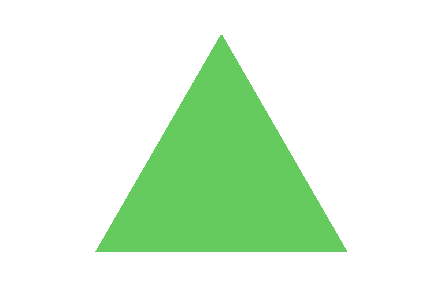
\includegraphics[width=0.3\textwidth]{img/dirichlet111.png}
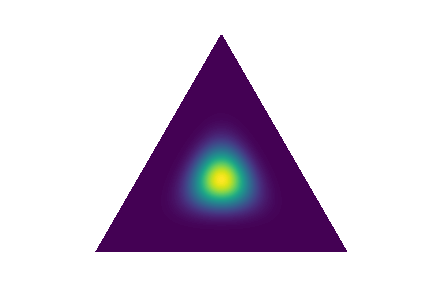
\includegraphics[width=0.3\textwidth]{img/dirichlet101010.png}
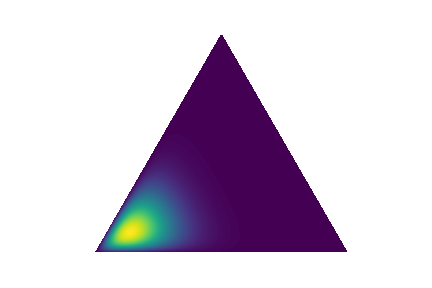
\includegraphics[width=0.3\textwidth]{img/dirichlet1022.png}
\caption{Distribuciones Dirichlet para $k=3$ con parámetros de concentración $\alpha$ (desde izquierda a derecha) dado por $[1,1,1]$, $[10,10,10]$ y $[10,2,2]$. }.
\label{fig:dist_Dirichlet}
\centering
\end{figure}


Veamos a continuación que la distribución de Dirichlet es conjugada al modelo Multinomial, y consecuentemente para Bernoulli, Categórica y Binomial. En efecto, si $\theta \sim \dir{\theta;\alpha}$ y $X\sim\mul{X;n,\theta}$, entonces

\begin{align}
	p(\theta|x) &= \frac{\mul{x;n,\theta}\dir{\theta;\alpha}}{p(x)}\nonumber\\
				&=  \frac{n!}{ x_1!\cdots x_k!p(x) B(\alpha)} \prod_{i=1}^k \theta_i^{x_i + \alpha_i-1}\nonumber\\
				&=  \frac{1}{B(\alpha')} \prod_{i=1}^k \theta_i^{\alpha'_i-1}
				\label{eq:dirichlet_post}
\end{align}
donde $\alpha' = (\alpha'_1,\ldots,\alpha'_k) = (\alpha'_1 + x_1,\ldots,\alpha'_k+ x_k)$ es el nuevo parámetro de concentración.

\begin{example}
	Consideremos $\alpha = [1,2,3,4,5]$ y generemos una muestra de $\theta\sim\dir{\theta|\alpha}$. El siguiente código genera, grafica e imprime esta muestra. 
	\begin{lstlisting}[language=Python]
	import numpy as np
	alpha = np.array([1,2,3,4,5]) 
	theta = np.random.dirichlet(alpha)
	plt.bar(np.arange(5)+1, theta);
	print(f'theta = {theta}')
\end{lstlisting}
En nuestro caso, obtuvimos los parámetros $ \theta = [0.034, 0.171, 0.286, 0.185, 0.324]$.

 Ahora, usaremos un prior Dirichlet sobre $\theta$ con $\alpha_p = [1,1,1,1,1]$ para calcular la posterior de acuerdo a la ecuación \eqref{eq:dirichlet_post}. La Figura \ref{fig:post_Dirichlet} muestra 50 muestras de la distribución posterior para distintas cantidades de observaciones entre 0 y  $ 10^5$. 

\begin{figure}[H]
\centering
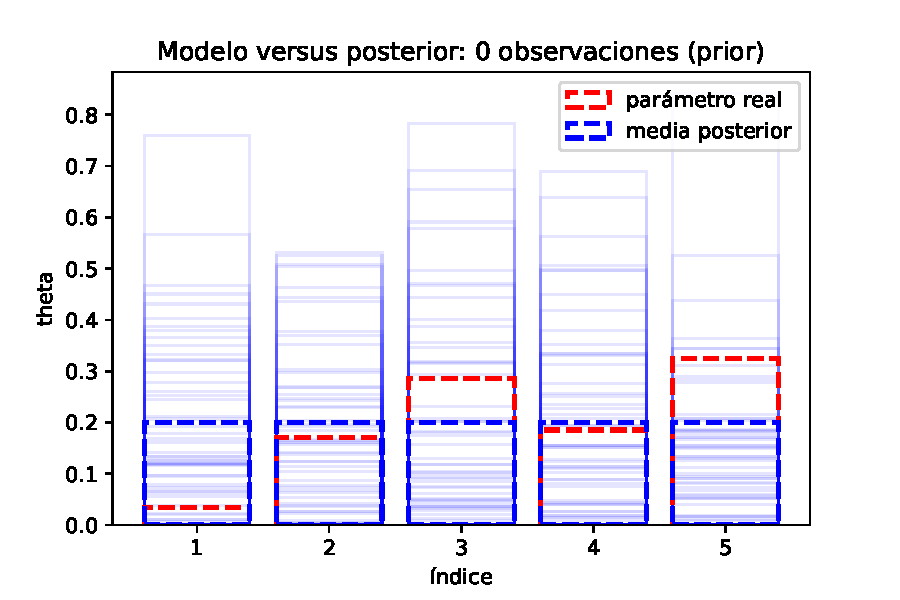
\includegraphics[width=0.3\textwidth]{img/post_dirichlet_0.pdf}
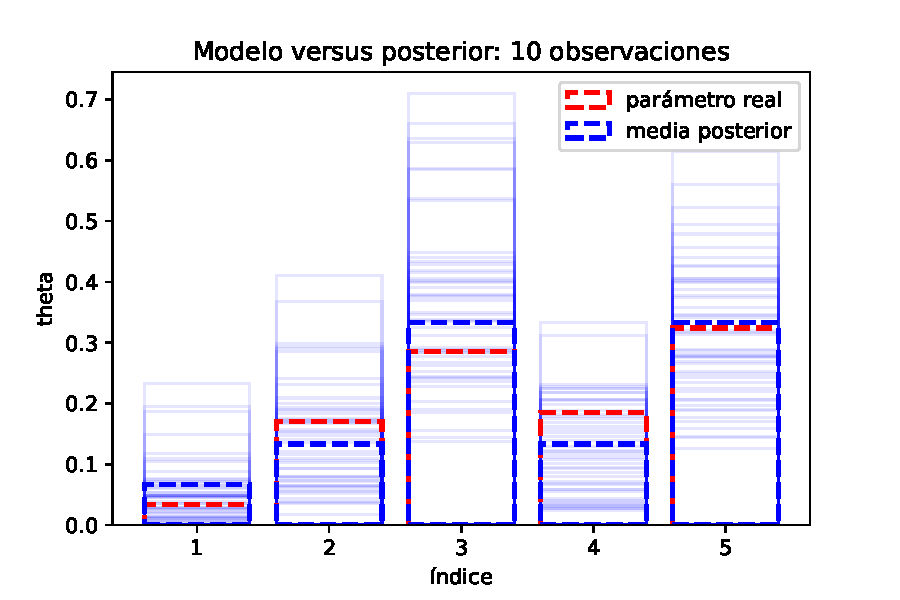
\includegraphics[width=0.3\textwidth]{img/post_dirichlet_10.pdf}
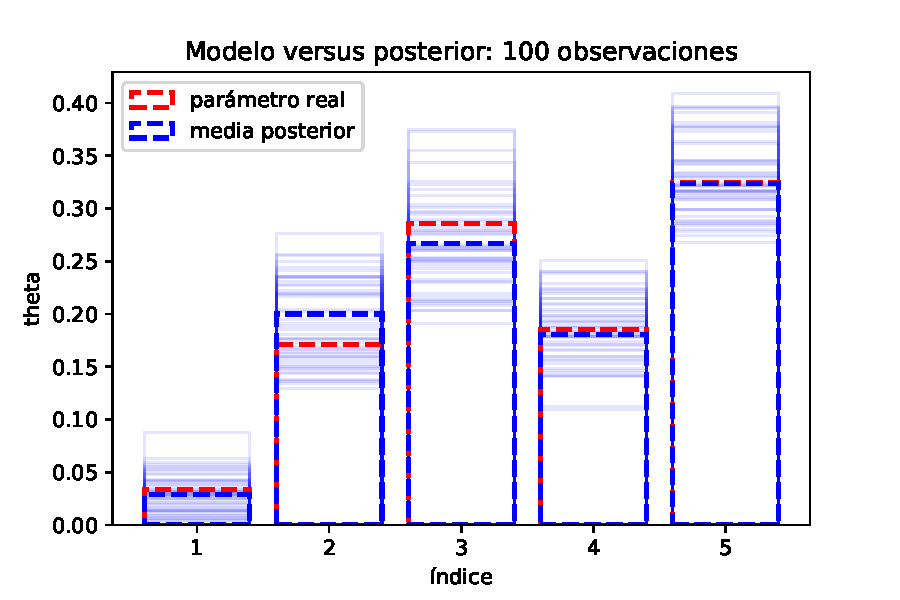
\includegraphics[width=0.3\textwidth]{img/post_dirichlet_100.pdf}\\
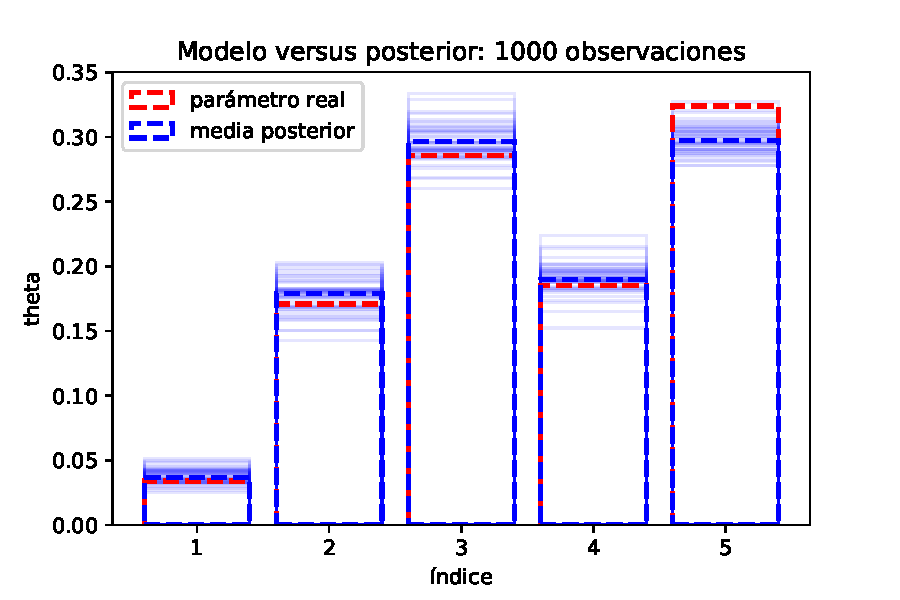
\includegraphics[width=0.3\textwidth]{img/post_dirichlet_1000.pdf}
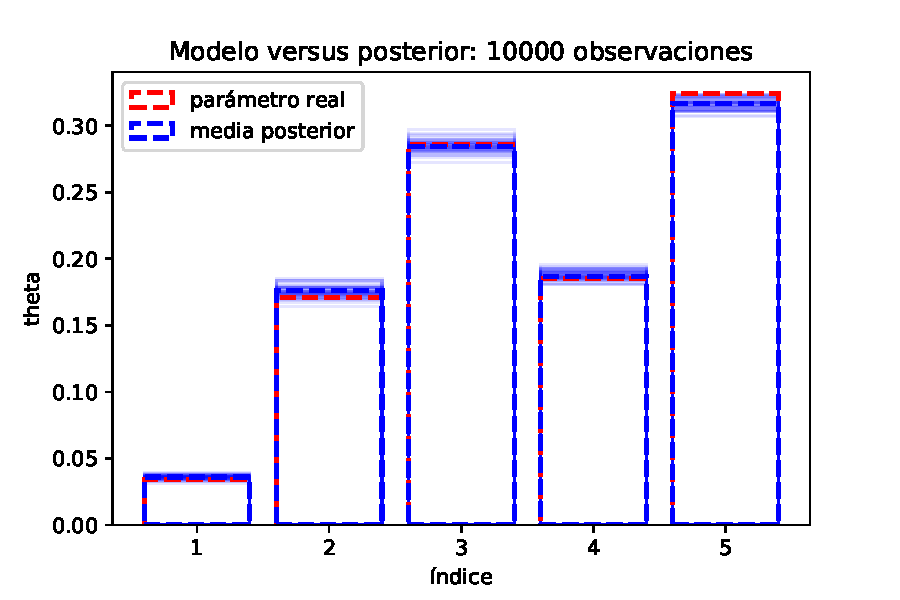
\includegraphics[width=0.3\textwidth]{img/post_dirichlet_10000.pdf}
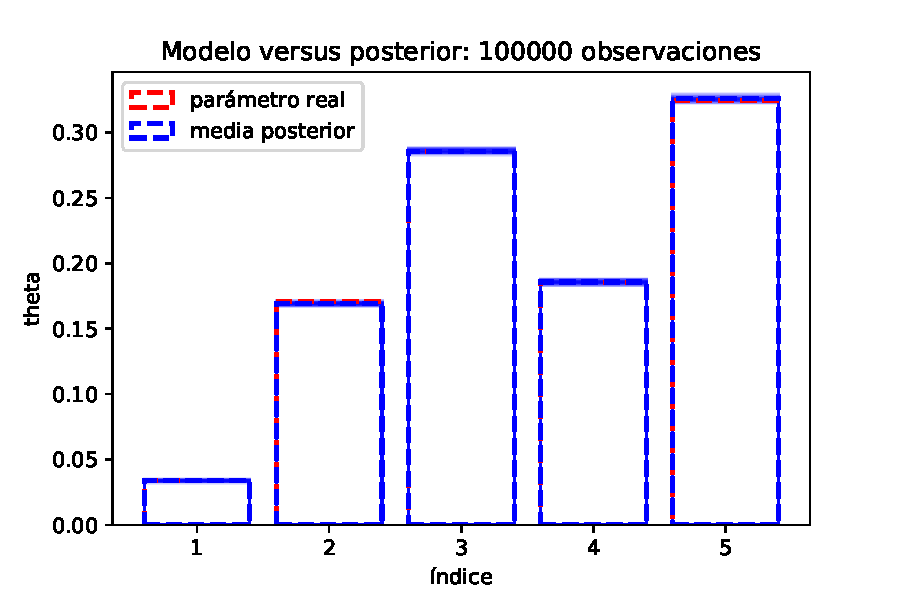
\includegraphics[width=0.3\textwidth]{img/post_dirichlet_100000.pdf}
\caption{Concentración de la distribución posterior en torno al parámetro real para un modelo $X\sim\mul{\theta}$ y una distribución a priori Dirichlet $\theta\sim\dir{\alpha}$. Se considera desde 0 hasta $10^5$ observaciones y cada gráfico (desde izquierda-arriba hasta derecha-abajo) muestra el parámetro real (linea roja quebrada), la media posterior (línea azul quebrada) y 50 muestras de la posterior (azul claro). Observe cómo la distribución a priori (línea azul quebrada en la primera figura) pierde importancia a medida que el número de observaciones aumenta.}
\label{fig:post_Dirichlet}
\end{figure}
\end{example}


\begin{example} \textbf{Modelo gaussiano ($\sigma^2$ conocido).} Consideremos el prior sobre la media $p(\mu) = \cN(\mu_0,\sigma_0^2)$, con lo que la posterior está dada por  
 \begin{align}
 	p(\mu|\mathcal{D}) &\propto \prod_{i=1}^n \frac{1}{\sqrt{2\pi\sigma^2}}\exp\left(-\frac{1}{2\sigma^2}(x_i-\mu)^2\right) \frac{1}{\sqrt{2\pi\sigma_0^2}}\exp\left(-\frac{1}{2\sigma_0^2}(\mu-\mu_0)^2\right)\label{eq:post_normal_mu_1}\\
 	&\propto \exp\left(-\frac{1}{2\sigma^2}\sum_{i=1}^n(x_i-\mu)^2-\frac{1}{2\sigma_0^2}(\mu-\mu_0)^2\right),\label{eq:post_normal_mu_2}
 \end{align} 
 donde la proporcionalidad viene de ignorar la constante $p(\mathcal{D})$ en la primera línea e ignorar todas las contantes que no dependen de $\mu$ en la segunda línea. Recordemos que estas constantes para $\mu$ incluyen a la varianza de $x$, $\sigma^2$, por lo que ignorar esta cantidad es solo posible debido a que estamos considerando el caso en que $\sigma^2$ es conocido. Completando la forma cuadrática para $\mu$ dentro de la exponencial en la ec.~\eqref{eq:post_normal_mu_2}, obtenemos
 \begin{equation}
 	p(\mu|\mathcal{D}) \propto \exp\left(-\frac{1}{2\sigma_n^2}(\mu - \mu_n)^2\right),\label{eq:post_normal_mu_3}
 \end{equation} 
 donde (ya definiremos $\mu_n$ y $\sigma_n^2$ en breve) como $p(\mu|\mathcal{D})$ debe integrar uno, la única densidad de probabilidad proporcional al lado derecho de la ecuación anterior es la Gaussiana de media $\mu_n$ y varianza $\sigma_n^2$. Es decir, la constante de proporcionalidad necesaria para la igualdad en la expresión anterior es
 \begin{equation}
     \int_\R\exp\left(-\frac{1}{2\sigma_n^2}(\mu - \mu_n)^2\right)\d\mu = (2\pi\sigma_n^2)^{n/2}.
 \end{equation} Consecuentemente, confirmamos que el prior elegido era efectivamente conjugado con la verosimilitud gaussiana, con lo que la posterior está dada por la siguiente densidad (gaussiana):
  \begin{equation}
 	p(\mu|\mathcal{D}) = \cN(\mu;\mu_n,\sigma_n^2) = \frac{1}{(2\pi\sigma_n^2)^{N/2}}\exp\left(-\frac{1}{2\sigma_n^2}(\mu - \mu_n)^2\right),\label{eq:post_normal_mu_4}
 \end{equation} 
 donde la media y la varianza están dadas respectivamente  por 
 \begin{align}
 	\mu_n &= \frac{1}{\tfrac{1}{\sigma_0^2} + \tfrac{n}{\sigma^2}} \left(\frac{1}{\sigma_0^2}\mu_0 + \frac{n}{\sigma^2}\bar{x} \right), \quad \text{donde } \bar{x} = \frac{1}{n}\sum_{i=1}^n x_i\label{eq:post_Gm}\\
 	\sigma_n &= \left(\frac{1}{\sigma_0^2} + \frac{n}{\sigma^2}\right)^{-1}.\label{eq:post_Gv}
 \end{align}
\end{example}
\begin{remark}
	La actualización bayesiana transforma los parámetros del prior de  $\mu$ desde  $\mu_0$ y $\sigma_0^2$ hacia $\mu_n$ y $\sigma_n^2$ en las ecs.~\eqref{eq:post_Gm} y \eqref{eq:post_Gv} respectivamente. Notemos que los  parámetros de la posterior son combinaciones (interpretables por lo demás) entre los parámetros del prior y los datos, en efecto, la $\mu_n$ es el promedio ponderado entre  $\mu_0$ (que es nuestro candidato para $\mu$ antes de ver datos) con factor $\sigma_0^{-2}$ y el promedio de los datos $\bar{x}$ con factor $(\sigma^{2}/n)^{-1}$, que a su vez es el estimador de máxima verosimilitud. Es importante también notar que  estos  factores son las varianzas inversas---i.e., precisión---de $\mu_0$ y de $\bar{x}$. Finalmente, observemos que $\sigma_n$ es la \emph{suma paralela} de las varianzas, pues  si expresamos la ec.~\eqref{eq:post_Gv} en términos de \emph{precisiones}, vemos que la precisión inicial $\sigma_0^2$ aumenta un término $\sigma^2$ con cada dato que vemos; lo cual tiene sentido pues con más información es la precisión la que debe aumentar y no la incertidumbre (en este caso representada por la varianza).
\end{remark}
\begin{example} \textbf{Modelo gaussiano ($\mu$ conocido).} Ahora procedemos con el siguiente prior para la varianza, llamado Gamma-inverso:
 \begin{equation}
 	p(\sigma^2)= \text{inv-}\Gamma(\sigma^2;\alpha,\beta) = \frac{\beta^\alpha}{\Gamma(\alpha) (\sigma^2)^{\alpha+1}}\exp(-\beta/\sigma^2)
 \end{equation}
 esta densidad recibe dicho nombre pues es equivalente a modelar la precisión, definida como el recíproco de la varianza $1/\sigma^2$, mediante la distribución Gamma. Los hiperparámetros $\alpha$ y $\beta$ son conocidos como parámetros de forma y de tasa (o precisión) respectivamente. 

 Con este prior, la posterior de la varianza toma la forma:
 \begin{align}
 	p(\sigma^2|\mathcal{D}) &\propto \prod_{i=1}^N \frac{1}{\sqrt{2\pi\sigma^2}}\exp\left(-\frac{1}{2\sigma^2}(x_i-\mu)^2\right) \frac{\beta^\alpha}{\Gamma(\alpha) (\sigma^2)^{\alpha+1}}\exp(-\beta/\sigma^2)\\
 	&\propto  \frac{1}{(\sigma^2)^{N/2+\alpha+1}}\exp\left(-\frac{1}{\sigma^2}\left(\frac{1}{2}\sum_{i=1}^N(x_i-\mu)^2 +\beta\right) \right)\nonumber
 \end{align} 
 donde nuevamente la proporcionalidad ha sido mantenida debido a la remoción de las constantes. Esta última expresión es proporcional a una distribución Gamma inversa con hiperparámetros $\alpha$ y $\beta$ ajustados en base a los datos observados. 


\end{example}




Hay ocasiones en las que el conocimiento a priori sobre el parámetro no puede ser convenientemente expresado mediante una densidad de probabilidad pero sí una densidad que no necesariamente integra uno o incluso es (Lebesgue) integrable. Para reflejar esta idea, se usan priors impropios.

\begin{definition}[Prior impropia] Una distribución a priori impropia es una distribución que no es necesariamente de probabilidad (i.e., no integra 1), pero que de todas formas puede ser utilizada como distribución a priori en el contexto de inferencia bayesiana, pues la distribución posterior correspondiente si es una distribución de probabilidad apropiada. 
\end{definition}

\begin{remark} No es necesario usar la constante de normalización en las densidades a priori Gaussianas (o ninguna otra en realidad).
\end{remark}

\begin{remark} Veamos que un prior impropio puede incluso tener integral infinita, en el caso de la distribución normal $X\sim\cN(X;\mu,1)$,  $\mu\in\R$, podemos elegir $p(\mu)\propto1$ y escribir 
\begin{equation}
	p(\mu|x)\propto p(x|\mu)\cdot 1 = \cN(x;\mu,1) = \cN(\mu;x,1). 
\end{equation}
	
\end{remark}

Considerar distribuciones uniformes impropias como priors no informativas parece tener sentido, pues intuitivamente no estamos dando preferencia (mayor probabilidad a priori) a ningún valor del parámetro por sobre otro. Sin embargo, este procedimiento sufre de una desventaja conceptual.


\section{Máxima Verosimilitud} % (fold)
\label{sec:estimador_de_máxima_verosimilitud}

Informalmente, el estimador de un parámetro es una función de los datos que deseamos que entregue un valor cercano al parámetro. Dada una cantidad desconocida, se hace natural la idea de buscar encontrar una \emph{buena} (y ojalá la \emph{mejor}) función de los datos que nos permita estimarla, pero ¿Qué significa que un estimador sea un buen estimador?

Dado que el parámetro $\theta$ es desconocido, calcular la distancia de un estimador $\hat\theta = \hat\theta(X)$ a este no es posible, pues de lo contrario  podríamos simplemente utilizar una función de pérdida como las definidas en el capítulo anterior.

En esta sección, veremos cómo construir estimadores usando directamente la densidad de probabilidad de la VA $X\in\cX$, donde aparece el parámetro $\theta$ y una colección de datos (o realizaciones del modelo). Para este fin la función de verosimilitud en la definición \ref{función_verosimilitud} será fundamental. Recordemos que la función de verosimilitud (del parámetro $\theta$ dados los datos $X$) es la densidad de probabilidad de los datos $X$ si el valor del parámetro fuese efactivamente $\theta$. Consecuentemente, la verosimilitud permite encontrar un estimador en base a una métrica clara: cuan probable es cada estimador de haber generado los datos. Esto da las condiciones para determinar un estimador que recibe mucha atención en la literatura estadística: 

\begin{definition}[Estimador de máxima verosimilitud (MV)]
	Sea una observación $x$ y una función de verosimilitud $L(\theta)$, el estimador de máxima verosimilitud está dado por 
	\begin{equation}
		\thetaMV = \underset{\theta}{\arg\max}\ L(\theta|x)
	\end{equation}	
\end{definition}

Claramente, el estimador de MV puede ser definido con respecto a la verosimilitud o a cualquier función no decreciente de ésta, como también pude no existir o no ser único. En particular, nos enfocaremos en encontrar $\thetaMV$ mediante la maximización de la log-verosimilitud $l(\theta) = \log L(\theta)$, la cual es usualmente más fácil de optimizar en términos computacionales o analíticos. De hecho, muchas veces incluso ignoraremos constantes de la (log) verosimilitud, pues éstas no cambian el máximo de $L(\theta)$.

\begin{example}[Máxima verosimilitud: Bernoulli]
	\label{ex:bernoulli_MV}
	Sea $X_1,\ldots X_n\sim\ber{\theta}$, la verosimilitud de $\theta$ está dada por 
	\begin{equation}
		L(\theta) = \prod_{i=1}^n\theta^x_i(1-\theta)^{1-x_i},
	\end{equation}
	y su log-verosimilitud por $l(\theta) = (\sum_{i=1}^nx_i)\log \theta + (n-\sum_{i=1}^nx_i)\log(1-\theta)$. El estimador de  MV puede ser encontrado resolviendo $\frac{\partial l(\theta)}{\partial \theta} = 0$:
	\begin{align*}
	\frac{\partial l(\theta)}{\partial \theta} =0 
	&\Rightarrow  (\sum_{i=1}^nx_i) \theta^{-1} = (n-\sum_{i=1}^nx_i)(1-\theta)^{-1}\\
	&\Rightarrow  \sum_{i=1}^nx_i (1-\theta) = (n-\sum_{i=1}^nx_i) \theta\\
	&\Rightarrow  \theta = \sum_{i=1}^nx_i/n.
	\end{align*}
Notemos que este estimador de MV ¡es a su vez el EIVUM!	
\end{example}


\begin{exercise}
	Graficar $l(\theta)$ en el Ejemplo \ref{ex:bernoulli_MV}.
\end{exercise}

\begin{exercise}
	Encuentre el estimador de MV de $\theta = (\mu,\Sigma)$ para la VA $X\sim\cN(\mu,\Sigma)$.
\end{exercise}

\begin{example}
	Sea la VA $X\sim\uni{\theta}$, es decir, $p(x) = \theta^{-1} \ind_{0\leq x \leq \theta}$. Para calcular la verosimilitud, recordemos en primer lugar que la verosimilitud factoriza de acuerdo a  
	\begin{equation}
		L(\theta) = \prod_{i=1}^n p_\theta(x_i)
	\end{equation}
	y observemos que necesariamente $p_\theta(x_i) = 0$ si $x_i>\theta$. Consecuentemente, $L(\theta)>0$ solo si $\theta$ es mayor que toda las observaciones, en particular, si $\theta\geq\max\{x_i\}_1^n$.

	Además, si efectivamente tenemos $\theta\geq\max\{x_i\}_1^n$, entonces notemos que $p_\theta(x_i) = 1/\theta$, por lo que la verosimilitud está dada por
		\begin{equation}
		L(\theta) = \theta^{-n}, \quad \theta\geq\max\{x_i\}_1^n
	\end{equation}
	y consecuentemente, el estimador de máxima verosimilitud es $\thetaMV = \max\{x_i\}_1^n$.
\end{example}

\section{EMV en práctica: tres ejemplos} % (fold)
\label{sub:MV_tres_ejemplos}

\subsection{Regresión lineal y gaussiana} 
\label{sub:reg_lin}


Una aplicación muy popular del estimador de MV es en los modelos de regresión lineal y gaussianos. Consideremos el caso donde se desea modelar la cantidad de pasajeros que mensualmente viajan en una aerolínea, para esto, sabemos de nuestros colaboradores en la división de análisis de datos de la aerolínea que ésta cantidad tiene una tendencia de crecimiento cuadrática en el tiempo y además una componente oscilatoria de frecuencia anual. Estos fenómenos pueden ser explicados por el aumento de la población, los costos decrecientes de la aerolínea y la estacionalidad anual de las actividades económicas. 

Asumiendo que la naturaleza de la cantidad de pasajeros es estocástica, podemos usar los supuestos anteriores para modelar la densidad condicional  de dicha cantidad (con respecto al tiempo $t$) mediante una densidad normal parametrizada de acuerdo a 
\begin{equation}
	X \sim \cN\left(\theta_0 + \theta_1 t^2 + \theta_2\cos(2\pi t/12), \theta_3^2\right),
\end{equation}
donde $\theta_0,\theta_1,\theta_2$ parametrizan la media y $\theta_3$ la varianza. 

Consecuentemente, si nuestras observaciones están dadas por $\{(t_i,x_i)\}_{i=1}^n$ podemos escribir la log-verosimilitud de $\theta$ como 
\begin{align}
	\label{eq:logV_ejemplo_reg}
	l(\theta) 	&=\loga{\prod_{i=1}^n \frac{1}{\sqrt{2\pi\theta_3^2}}\expo{-\frac{(x_i-\theta_0 - \theta_1 t^2 - \theta_2\cos(2\pi t/12))^2}{2\theta_3^2}}}\nonumber \\
	&=\frac{n}{2}\loga{2\pi\theta_3^2}  - \frac{1}{2\theta_3^2}\sum_{i=1}^n (x_i - \theta_0 - \theta_1 t_i^2 - \theta_2\cos(2\pi t_i/12))^2
\end{align}
con lo que vemos que $\thetaMV$ puede ser calculado explícitamente y es función de $\{(t_i,x_i)\}_{i=1}^n$ debido a que la ecuación \eqref{eq:logV_ejemplo_reg} es cuadrática en $[\theta_0,\theta_1,	\theta_2]$.


% subsection estimador_de_mv_en_la_práctica_tres_ejemplos (end)

\subsection{Regresión no lineal: clasificación} 
\label{sub:clasif}

La razón por la cual $\thetaMV$ pudo ser calculado de forma explícita es porque el modelo Gaussiano con media parametrizada de forma lineal resulta en una log-verosimilitud cuadrática, donde el mínimo es único y explícito. Sin embargo, en muchas situaciones el modelo lineal y gaussiano no es el apropiado. 

Un ejemplo es esto es problema de evaluación crediticia (\textit{credit scoring}) donde en base a un conjunto de \textit{características} que definen a un cliente, un ejecutivo bancario debe evaluar si otorgarle o no el crédito que el cliente solicita. Para tomar esta decisión, el ejecutivo puede revisar la base de datos del banco e identificar los clientes que en el pasado pagaron o no pagaron sus créditos para determinar el perfil del \textit{pagador} y el del \textit{no-pagador}. Finalmente, un nuevo cliente puede ser \textit{clasificado} como pagador/no-pagador en base su similaridad con cada uno de estos grupos. 

Formalmente, denotemos las características del cliente como $t\in\R^N$ y asumamos que el cliente paga su crédito con probabilidad $\sigma(t)$ y no lo paga con probabilidad $1- \sigma(t)$, la función $\sigma(t)$ a definir. Esto es equivalente a construir la VA $X$
\begin{equation}
 	X|t \sim \ber{\sigma(t)}
 \end{equation} 
 donde $X=1$ quiere decir que el cliente paga su crédito y $X=0$ que no. Una elección usual para la función $\sigma(\cdot)$ es la función logística aplicada a una transformación lineal de $t$, es decir, 
 \begin{equation}
 	\Pr{(X=1|t)} = \frac{1}{1+e^{-(\theta_0 + \theta_1 t)	}}.
 \end{equation}
Notemos que este es un clasificador lineal, donde $\theta = [\theta_0, \theta_1]$ define un hiperplano en $\R^N$ en donde los clientes $t\in\{t | 0\leq \theta_0 + \theta_1 t\}$ pagan con probabilidad mayor o igual a 1/2 y el resto con probabilidad menor o igual a 1/2. Esto es conocido como \textbf{regresión logística}. 

Entonces, usando los registros bancarios $\{(x_i,t_i)\}_{i=1}^n$ ¿cuál es el $\theta = [\theta_0, \theta_1]$ de máxima verosimilitud? Para esto notemos que la log-verosimilitud puede ser escrita como 
\begin{align*}
	l(\theta) &= \log \prod_{i=1}^n p(x_i|t) \\
			  &= \sum_{i=1}^n x_i \log \sigma(t) + \left(n-\sum_{i=1}^n x_i\right)\log(1-\sigma(t))\\
			  &= \sum_{i=1}^n x_i \log \frac{1}{1+e^{-(\theta_0 + \theta_1 t)	}} + \left(n-\sum_{i=1}^n x_i\right)\log(1-\frac{1}{1+e^{-(\theta_0 + \theta_1 t)	}})
\end{align*}
Esta expresión no tiene mínimo global y a pesar que podemos calcular su gradiente, no podemos resolver $\partial l(\theta)/\partial \theta =0$ de forma analítica, por lo que debemos usar métodos de descenso de gradiente.  

\subsection{Variables latentes: \textit{Expectation-Maximisation}} 
\label{sub:EM}

En ciertos escenarios es natural asumir que nuestros datos provienen de una mezcla de modelos, por ejemplo, consideremos la distribución de estaturas en una población, podemos naturalmente modelar esto como una mezcla de distribuciones marginales para las estaturas de hombres y mujeres por separado, es decir, 
\begin{equation}
	X\sim p\cN(X|\mu_H,\Sigma_H) + (1-p)\cN(X|\mu_M,\Sigma_M)
\end{equation}
donde la verosimilitud de los parámetros $\theta = [p, \mu_H, \sigma_H,, \mu_M, \sigma_M]$ dado un conjunto de observaciones $\{x_i\}_{i=1}^n$ es
\begin{align*}
	L(\theta) 	&= \prod_{i=1}^n \left( p\cN(X|\mu_H,\Sigma_H) + (1-p)\cN(X|\mu_M,\Sigma_M) \right)\\
				&= \prod_{i=1}^n \left( p\frac{1}{\sqrt{2\pi\Sigma_H^{-1}}}\expo{\frac{-(x_i-\mu_H)^2}{2\Sigma^2_H}} + (1-p)\frac{1}{\sqrt{2\pi\Sigma_M^{-1}}}\expo{\frac{-(x_i-\mu_M)^2}{2\Sigma^2_M}}\right).
\end{align*}
Optimizar esta expresión con respecto a las 5 componentes de $\theta$ es difícil, en particular por la suma en la expresión, lo cual no permite simplificar la expresión mediante la aplicación de $\log(\cdot)$. 

Una interpretación de la diferencia de este modelo con respecto a los anteriores es la introducción implícita de una  \textit{variable latente} que describe de qué gaussiana fue generada cada observación. Si conociésemos esta variable latente, el problema sería dramáticamente más sencillo. En efecto, asumamos que tenemos a nuestra disposición las observaciones $\{z_i\}_{i=1}^n$ de la VA $\{Z_i\}_{i=1}^n$ las cuales denota de qué modelo es generada cada observación, por ejemplo, $Z_i=0$ (cf. $Z_i=1$) denota que el individuo con estatura $X_i$ es hombre (cf.~mujer).
 
En este caso, asumamos por un segundo que estas variables latentes están disponibles y consideremos los \textbf{datos completos} $\{(x_i,z_i)\}_{i=1}^n$ para escribir la función de verosimilitud completa mediante
\begin{align*}
	l(\theta|z_i,x_i) &= \prod_{i=1}^n \cN(X|\mu_H,\Sigma_H)^{z_i} \cN(X|\mu_M,\Sigma_M)^{(1-z_i)}\\
	&\hspace{-3em}= \sum_{i=1}^n \left( z_i\log\frac{1}{\sqrt{2\pi\Sigma_H^{-1}}}\expo{\frac{-(x_i-\mu_H)^2}{2\Sigma^2_H}} + (1-z_i)\log\frac{1}{\sqrt{2\pi\Sigma_M^{-1}}}\expo{\frac{-(x_i-\mu_M)^2}{2\Sigma^2_M}}\right).
\end{align*}
Esta función objetivo es mucho más fácil de optimizar, pero no es observable pues la VA $Z$ es desconocida. Una forma de resolver esto es tomando la esperanza condicional de la expresión anterior (con respecto a $Z$) condicional a los datos y los parámetros \textit{actuales}, para luego maximizar esta expresión c.r.a. $\theta$ y comenzar nuevamente. Específicamente, como la expresión anterior es lineal en $z_i$ basta con tomar su esperanza: 
\begin{align*}
	\Et{Z_i|\theta_t,x_i} &= 1\cdot\Prob{Z_i=1|\theta_t,x_i} + 0\cdot\Prob{Z_i=0|\theta_t,x_i}\\
	&= 	\frac{\Prob{x_i|\theta_t,z_i=1} p(z_i=1)}{p(x_i|\theta)}\\
	&= 	\frac{\Prob{x_i|\theta_t,z_i=1} p(z_i=1)}{p(x_i|z=1,\theta)p(z=1)+p(x_i|z=0	,\theta)p(z=0)}
\end{align*}









\section{Propiedades del EMV} 
\label{sec:propiedades_EMV}
\subsection{Consistencia} 

La primera propiedad que veremos del EMV es su consistencia. Que un estimador $\hat\theta$ sea \textit{consistente} quiere decir que éste tiende (de alguna forma) al parámetro real $\theta$ a medida vamos considerando más datos. Definamos en primer lugar la siguiente \emph{divergencia}.

\begin{definition}[Divergencia de Kullback-Liebler]
Para dos densidades de probabilidad $f$ y $g$, definidas sobre un mismo conjunto de partida $\cX$, la divergencia de Kullback-Leibler entre ellas está definida mediante 
\begin{equation}
	\KL{f}{g} = \int_\cX f(x)\loga{\frac{f(x)}{g(x)}}\dx.
\end{equation}
\end{definition}

\begin{remark} La divergencia KL es siempre positiva $\forall f,g$ (desigualdad de Gibbs):
\begin{align*}
 	-\KL{f}{g}  &= \int_\cX f(x)\loga{\frac{g(x)}{f(x)}}\dx\\
 				&\leq \loga{\int_\cX f(x)\frac{g(x)}{f(x)}}\dx, \quad\quad \text{(Jensen's)}\\
 				&= \loga{\int_\cX g(x)}\dx\\
 				&=\log 1=0.,	
 \end{align*} 
Adempás, como $\log(\cdot)$ es estrictamente convexo, la igualdad $\KL{f}{g}=0$ solo se cumple si el argumento $\frac{g(x)}{f(x)}$ es constante, lo cual se tiene solo para ${g(x)} = {f(x)}$.
\end{remark}

\begin{remark} Intuición y gráfico de la KL en relación al soporte.
\end{remark}

\begin{remark} Intuición de la KL desde la teoría de la información (entropía).
\end{remark}



Otra propiedad clave de la divergencia KL es que puede ser infinita y es asimétrica, por esta razón nos referimos a KL como divergencia y no \emph{distancia}. La intuición detrás de la KL es que es una medida de \textit{error} de estimar la densidad $f$ mediante la densidad $g$. 

 Con la KL, definiremos que un modelo/parámetro es \textbf{identificable} si los valores para los parámetros $\theta\neq\theta'$ implican $\KL{p_\theta}{p_\theta'}>0$, lo que significa que distintos valores del parámetro dan origen a distintos modelos, intuitivamente, esto significa que la \emph{parametrización} del modelo estadístico no es redundante. Asumiremos desde ahora que los modelos considerados son identificables.

El estimador de MV puede ser obtenido de la maximización de
\begin{equation}
\label{eq:Mn}
 	M_n (\theta') = n^{-1} (l_n(\theta') - l_n(\theta))  = \frac{1}{n} \sum_{i=1}^n \loga{\frac{p_{\theta'}(x_i)}{p_{\theta}(x_i)}},
 \end{equation} 
 donde $n$ es la cantidad de observaciones $\{x_1,\ldots,x_n\}$, $\theta$ es el parámetro real y $l_n(\cdot)$ es la log-verosimilitud en base a dichas observaciones. La obtención del EMV desde la maximización de $M_n (\theta')$ en la ecuación \eqref{eq:Mn} es posible porque $l_n(\theta)$ es constante para $\theta'$, con lo que $l_n(\theta')\propto_{\theta}M_n (\theta')$. 
 
 Entonces, gracias a la ley de los grandes números, tenemos que 
 \begin{equation}
 	M_n(\theta') \rightarrow \Et{\loga{\frac{p_{\theta'}(x)}{p_{\theta}(x)}}} = -\Et{\loga{\frac{p_{\theta}(x)}{p_{\theta'}(x)}}} = -\KL{p_\theta}{p_{\theta'}}.
 \end{equation}

 Consecuentemente, como el objetivo del estimador de MV tiende a la KL negativa, entonces maximizar la verosimilitud es equivalente a minimizar la KL-divergencia entre el modelo real y el modelo generado por el parámetro. 
\begin{remark}
 Máxima verosimilitud es (asintóticamente) efectivavamente equivalente a minimizar discrepancias en el espacio de modelos.
\end{remark}
 
\begin{remark}
 Si el modelo obtenido mediante MV tiende efectivamente al modelo real (no tenemos garantías de esto todavía) nuestro supuesto de \textit{identificabilidad} implica que el estimador de MV tiende al parámetro real también. Sin embargo, si el modelo está parametrizado de tal forma que no es identificable, convergencia en el espacio de modelos no implica necesariamente convergencia en los parámetros.   
\end{remark}
 
 


 Otra propiedad muy utilizada en la práctica es el \textbf{Principio de equivarianza}, el cual establece que si $\thetaMV$ es el estimador de MV de $\theta$, entonces, $g(\thetaMV)$ es el estimador de MV del parámetro transformado $g(\theta)$.

\begin{example}(Cálculo del EMV en Gaussiana: varianza versus precisión versus log-precisión versus cholesky - reparametrisation trick)
	
\end{example}

\subsection{Normalidad asintótica}

Otra propiedad es la \textbf{normalidad asintótica del EMV}, esto significa que el estimador ML (como cantidad aleatoria) es normal en el límite que la cantidad de  observaciones tiende a infinito. 

Para entender esta propiedad, primero definamos la función de puntaje o \textit{score function} como la {función aleatoria} definida por la derivada de la log-verosimilitud, es decir, 
\begin{equation}
	S_\theta(X) = \frac{\partial \log p_\theta(X)}{\partial\theta}.
\end{equation}

\begin{remark}
La esperanza de la función de puntaje cero. En efecto, derivando la igualdad fundamental $1 = \int_\cX p_\theta(x)\dx$ con respecto a $\theta$, obtenemos 
\begin{align}
	0 = \int_\cX \frac{\partial  p_\theta(X)}{\partial\theta} \dx = \int_\cX \frac{1}{p_\theta(X)}\frac{\partial  p_\theta(X)}{\partial\theta} p_\theta(X) \dx = \int_\cX \frac{\partial \log   p_\theta(X)}{\partial\theta} p_\theta(X) \dx = \Et{S_\theta(X)}
\end{align}
Sorprendente. 
\end{remark}

Además, veamos que al derivar por segunda vez la función de puntaje, obtenemos: 
\begin{align*}
	0 &= \int_\cX \frac{\partial}{\partial \theta }\left(\frac{\partial \log   p_\theta(X)}{\partial\theta} p_\theta(X) \right)\dx\\ 
	&= \int_\cX \left(\frac{\partial^2 \log   p_\theta(X)}{\partial\theta^2} p_\theta(X) + \frac{\partial \log   p_\theta(X)}{\partial\theta}\frac{\partial   p_\theta(X)}{\partial\theta}  \right)\dx\\
	&= \Et{\frac{\partial^2 \log   p_\theta(X)}{\partial\theta^2}} + \Et{\left(\frac{\partial \log   p_\theta(X)}{\partial\theta}\right)^2}.
\end{align*}
Cada uno de los dos términos de la ecuación anterior tiene la misma magnitud (uno es negativo y el otro es positivo), lo cual motiva la siguiente definición.

\begin{definition}[Información de Fisher]
La cantidad denotada mediante  
\begin{equation}
		I(\theta) = \Et{\left(\frac{\partial \log   p_\theta(X)}{\partial\theta}\right)^2} = 	-\Et{\frac{\partial^2 \log   p_\theta(X)}{\partial\theta^2}},
\end{equation}	
es conocida como información de Fisher. Además, como la esperanza de la función de puntaje es cero, la varianza de $I(\theta)$ puede ser expresada como 
\begin{equation}
	\Vt{S_\theta(X)} = \Et{S_\theta(X)^2} - \cancel{\Et{S_\theta(X)}^2} = \Et{\left(\frac{\partial \log   p_\theta(X)}{\partial\theta}\right)^2}.
\end{equation}
Consecuentemente, la información de Fisher también es la varianza de la función de pérdida, con lo que contamos con tres expresiones para poder calcular $I(\theta)$. 
\end{definition}

\begin{exercise}[Cálculo de la información de Fisher para Bernoulli]
	Consideremos $X\sim\ber{\theta}$, entonces, 
	\begin{align}
		I(\theta) &= -\Et{\frac{\partial^2}{\partial\theta^2}\loga{\theta^X(1-\theta)^{1-X}}}\nonumber\\
		&= -\Et{\frac{\partial^2}{\partial\theta^2} X\log\theta + \frac{\partial^2}{\partial\theta^2} 	(1-X)\loga{1-\theta}	}\nonumber\\
		&= \Et{X\theta^{-2} + (1-X)(1-\theta)^{-2}	}\nonumber\\
		&= \theta^{-1} + (1-\theta)^{-1}	\nonumber\\
		&= 	\frac{1}{\theta(1-\theta)}.
	\end{align}
\end{exercise}

\begin{exercise}[Cálculo de la información de Fisher para Poisson]
	Consideremos $X\sim\poi{\theta}$, entonces, 
	\begin{align}
		I(\theta) &= \Et{\left(\frac{\partial}{\partial\theta}\loga{\frac{\theta^Xe^{-\theta}}{X!}}\right)^2}\nonumber	\\
		&= \Et{\left( \frac{\partial}{\partial\theta}X\log\theta - \frac{\partial}{\partial\theta}\theta - \frac{\partial}{\partial\theta}\log(X!)\right)^2}\nonumber\\
		&= \Et{\left( X\theta^{-1} - 1\right)^2}\nonumber	\\
		&= \Et{ X^2\theta^{-2} -2X\theta^{-1}+ 1}\nonumber	\\
		&= (\theta+\theta^2)\theta^{-2} -2\theta\theta^{-1}+ 1\nonumber\\
		&= \theta^{-1}.\nonumber	
	\end{align}
\end{exercise}

Hasta ahora hemos calculado la función de puntaje en base a la verosimilitud de solo una una variable aleatoria. Si considerásemos la verosimilitud evaluada calculada para un conjunto de observaciones (IID), tenemos que
\begin{equation}
	S_\theta(X_1,\ldots,X_n) = \frac{\partial \log \prod_{i=1}^np_\theta(X_i)}{\partial\theta} = \sum_{i=1}^n\frac{\partial \log p_\theta(X_i)}{\partial\theta}= \sum_{i=1}^n S_\theta(X_i).
\end{equation}
De igual forma, para la información de Fisher, tenemos, 
\begin{equation}
	I_n(\theta) = \Vt{\sum_{i=1}^n S_\theta(X_i)} = n I(\theta).
\end{equation}
\begin{remark}
La expresión anterior confirma la intuición sobre la información de Fisher en cuanto a \emph{cuán informativa} es una muestra $X$ para estimar el parámetro $\theta$: Si una muestra tiene tiene una información de Fisher $I(\theta)$, entonces $n$ muestras independientes del mismo modelo tendrán  $n$ veces dicha información. 
\end{remark}

Veamos ahora una desigualdad interesante para la información de Fisher y su relación con estimadores. Consideremos un estimador insesgado, es decir, 
\begin{equation}
	\Et{\hat{\theta}(X)-\theta}=\int_\cX (\hat{\theta}(X)-\theta)p_\theta(X)\dx=0.
\end{equation}
Derivando esta expresión con respecto a $\theta$, obtenemos

\begin{align*}
	0 &= \frac{\partial}{\partial\theta}\int_\cX (\hat{\theta}(X)-\theta)p_\theta(X)\dx\\
	  &= -\int_\cX p_\theta(X)\dx  + \int_\cX (\hat{\theta}(X)-\theta)\frac{\partial p_\theta(X)}{\partial\theta}\dx\\
	  &= -1  + \int_\cX (\hat{\theta}(X)-\theta)\frac{\partial\log p_\theta(X) }{\partial\theta}p_\theta(X)\dx.
\end{align*}
Lo que implica que 
\begin{align*}
	1 &= \left(\int_\cX (\hat{\theta}(X)-\theta)\frac{\partial\log p_\theta(X) }{\partial\theta}p_\theta(X)\dx\right)^2\\
	&=\left(\int_\cX (\hat{\theta}(X)-\theta)\sqrt{p_\theta(X)}\sqrt{p_\theta(X)}\frac{\partial\log p_\theta(X) }{\partial\theta}\dx\right)^2\\
	&\leq\int_\cX (\hat{\theta}(X)-\theta)^2 p_\theta(X)\dx \int\left(\frac{\partial\log p_\theta(X) }{\partial\theta}\right)^2 p_\theta(X)\dx.
\end{align*}
Notemos que la primera integral es la varianza del estimador insesgado $\hat\theta$ y la segunda es la esperanza del cuadrado de la función de puntaje (o la información de Fisher). Con esto, podemos enunciar el siguiente resultado 
\begin{definition}[Cota de Cramer-Rao]
	Sea $X_1,\ldots,X_n \sim p_\theta$ y $nI(\theta)$ su información de Fisher. Entonces para todo estimador insesgado $\theta'$ tenemos 
	\begin{equation}
		\Vt{\theta'}\geq (nI(\theta))^{-1},\quad \forall \theta\in\Theta
	\end{equation}
\end{definition}
La cota de Cramer-Rao es un elemento fundamental en el estudio estadístico, pues establece que cualquier estimador tiene necesariamente una varianza que está por sobre el recíproco de la información de Fisher. 

Ahora podemos finalmente volver al concepto de normalidad asintótica. Si tenemos una colección de VA $X_1,\ldots,X_n\sim p_\theta$ con $\theta$ el parámetro real, entonces, la secuencia de estimadores de MV, $\thetaMV^{(n)}$ cumple con 
\begin{equation}
	\sqrt{n}(\thetaMV^{(n)}-\theta)\rightarrow \cN(0,(I(\theta))^{-1}),
\end{equation}
lo cual intuitivamente corresponde a que, para $n$ suficientemente grande, el estimador de MV está distribuido de forma normal en torno al parámetro real con varianza $(nI(\theta))^{-1}$. Lo que implica también \textit{eficiencia asintótica}: si $n$ es suficientemente grande, entonces la distribución del estimador es normal y su varianza tiende a cero. 

\section{Estimación y predicción}

\subsection{Estimadores bayesianos}

Si bien ya hemos estudiado el rol del prior en la inferencia bayesiana, hasta ahora no lo hemos considerado en la construcción de estimadores. En particular, el EMV no incorpora conocimiento a priori del parámetro. Con el objetivo de incorporar este conocimiento a priori en el cálculo de estimadores puntales, definimos el siguiente estimador bayesiano: 

\begin{definition}[Estimador máximo a posteriori]
Sea $\theta \in \Theta$ un parámetro con distribución a posteriori $p(\theta |D)$ definida en todo $\Theta$. Entonces nos referiremos a su estimación puntual dada por: 
$$
\theta_{MAP}= \underset{\Theta}{\arg\max}\ p(\theta|D),
$$
como el estimador \emph{máximo a posteriori} (MAP). 
\end{definition}

\begin{remark}
Es posible encontrar el MAP solo teniendo acceso a una versión \emph{proporcional} a la distribución posterior, un escenario usual en inferencia bayesiana, o también mediante la maximización del logaritmo de ésta última. En efecto, 
$$
\theta_{MAP} = \underset{\theta \in \Theta}{\arg\max }\ p(\theta|\mathcal{D}) = \underset{\theta \in \Theta}{\arg\max }\ p(\mathcal{D}|\theta)p(\theta)= \underset{\theta \in \Theta}{\arg\max}\left(\underbrace{\log p(\mathcal{D}|\theta)}_{l(\theta)} + \log p(\theta)\right),
$$
donde hemos encontrado la maximización de  la función de log-verosimilitud, pero ahora junto al log-prior.
\end{remark}

\begin{remark}
Es relevante notar que el estimador MAP es una \emph{modificación} del EMV, pues ambos comparten una parte de la misma función objetivo (verosimilitud) con la diferencia que el MAP además incluye el término \emph{log-prior}. Esto puede entenderse como una regularización de la solución del problema de MV, en donde el término adicional puede representar las propiedades del estimador más allá de que las pueden ser exclusivamente revelada por los datos. 
\end{remark}

\begin{example}[Máximo a posterior para el modelo gaussiano]
En particular, para el modelo lineal y gaussiano que hemos considerado hasta ahora, podemos calcular $\theta_{MAP}$ para un prior Gaussiano de media cero y varianza $\sigma_\theta^2$. Éste está dado por (asumimos la varianza del ruido $\sigma_\epsilon^2$ conocida):	
\begin{align}
	\theta_\text{MAP}^\star 	&= \text{argmax } p(Y|\theta,X)p(\theta)\nonumber\\
	\text{[ind., def.]}\ &= \text{argmax } \prod_{i=1}^N \cN(y_i;\theta^\top x_i,\sigma_\epsilon^2)\cN(\theta;0,\sigma_\theta^2) \nonumber\\
	&= \text{argmax } \prod_{i=1}^N \frac{1}{\sqrt{2\pi}\sigma_\epsilon} \exp\left({\frac{-1}{2\sigma_\epsilon^2}(y_i-\theta^\top x_i)^2}\right)											\frac{1}{(\sqrt{2\pi}\sigma_\theta)^{M+1}} \exp\left({\frac{-||\theta||^2}{2\sigma_\theta^2}}\right) \nonumber\\
	 &= \text{argmax } \frac{1}{\sqrt{2\pi}\sigma_\epsilon} \frac{1}{(\sqrt{2\pi}\sigma_\theta)^{M+1}} \exp\left( \sum_{i=1}^N{\frac{-1}{2\sigma_\epsilon^2}(y_i-\theta^\top x_i)^2} -{\frac{||\theta||^2}{2\sigma_\theta^2}}\right) \nonumber\\
	\text{[log.]}\  &= \text{argmin } \sum_{i=1}^N{(y_i-\theta^\top x_i)^2} +{\frac{\sigma_\epsilon^2}{\sigma_\theta^2}||\theta |^2}.\nonumber 
	\label{eq:MAP_reg_lin}
\end{align}
Podemos ver que eligiendo un prior uniforme o de normal de varianza muy amplia, el MAP es equivalente al EMV. ¿qué significa esto? ¿qué comportamiento differente de EMV promueve el MAP en este caso?
\end{example}

En el caso general, podemos considerar otros estimadores puntuales a través de una función de pérdida asociada a estimar el parámetro $\theta$ mediante el estimador $\hat\theta$ dada por $L(\theta,\hat\theta)$. Con esto podemos definir los conceptos de riesgo y estimador bayesiano.
\begin{definition}[Riesgo bayesiano]
Para una función de pérdida $L(\theta,\hat\theta)$ y un conjunto de observaciones $\cD$, el riesgo bayesiano es la esperanza posterior de dicha función de pérdida, es decir
\begin{equation}
    R(\hat\theta) = \int_\Omega L(\theta,\hat\theta)p(\theta|\cD)\d\theta.
\end{equation}
\end{definition}



\begin{definition}[Estimador bayesiano]
Dado un conjunto de datos $\cD$ y un riesgo bayesiano $R(\theta)$, un estimador bayesiano es uno que minimiza el riesgo bayesiano:
\begin{equation}
    \theta_\text{Bayes} = \arg\min_{\Omega} R(\theta).
\end{equation}
\end{definition}

\begin{example}
El  caso estándar es la función de pérdida cuadrática $L_2(\theta,\hat\theta) = (\theta-\hat\theta)^2$ la cual resulta en el estimador dado por la media posterior $\theta_\text{Bayes} = \E{\theta|\cD}$. De forma similar,la función de costo \emph{lineal} $L_1(\theta,\hat\theta) = |\theta-\hat\theta|_1$ resulta en el estimador dado por la mediana posterior. 
\end{example}

Encontrar una función de pérdida para el máximo a posteriori es menos directo. Consideremos en primer lugar el caso $\theta\in\Omega$ discreto y la pérdida ``0-1''
\[   
L_\text{0-1}(\theta,\hat\theta) = 
     \begin{cases}
       0 &\quad\text{si } \theta = \hat\theta,\\
       1 &\quad\text{si no}. 
     \end{cases}
\]

El riesgo de Bayes asociado a $L_\text{0-1}(\theta,\hat\theta)$ (en el caso discreto) toma la forma
\begin{equation}
    R(\hat\theta) = \Prob{\theta\neq\hat\theta|\cD} = 1-\Prob{\theta = \hat\theta|\cD},
\end{equation}
lo cual es minimizado eligiendo $\hat\theta$ tal que $\Prob{\theta = \hat\theta|\cD}$ es máximo, es decir, el MAP. ¿por qué no es posible proceder de esta forma para el caso continuo? ¿cuál es la función de costo asociada al MAP en el caso continuo?




\subsection{Posterior predictiva}

En la inferencia bayesiana las predicciones ocupan un rol relevante, pues luego de realizar inferencia sobre un modelo estadístico, en general estamos interesados estudiar cómo serán los siguientes datos genearados por el modelo. Para esto definiremos la predicción bayesiana de la forma

\begin{definition}[Posterior predictiva]
Para un conjunto de datos $\cD$ y un parámetro $\theta$, la densidad posterior predictiva está dada por
\begin{equation}
    p(x|\cD) = \int_\Omega p(x|\theta)p(\theta|\cD)\d\theta = \E{p(x|\theta) |\cD},
\end{equation}
es decir, el valor esperado del modelo estadístico con respecto a la ley posterior del parámetro (modelo).
\end{definition}
Podemos ahora considerar la posterior predictiva como nuestro modelo \emph{aprendido} y generar datos de él, donde nos encontramos frente al mismo dilema de un estimador puntual como en el caso anterior: es posible considerar muestras aleatorias, la media, la mediana o algún intervalo. 

\begin{remark}
La posterior predictiva es distinta (en general) a la predicción \emph{plug-in}, en donde consideramos en modelo estadístico $p_{\hat\theta}$ en base a un estimador (puntual) cualquiera $\hat\theta$. Desde esa perspectiva, la posterior predictiva equivale a considerar estimadores y modelos puntuales pero integrar todos ellos con respecto a la ley posterior. 
\end{remark}

\newpage


\section{El prior de Jeffreys}

Consideremos $X\sim p(x|\theta)$, $\theta \in [a,b]$, en donde elegimos el prior \textit{no informativo} uniforme dado por 
$$
	p(\theta) =\uni{a,b} = \frac{1}{b-a}.
$$
Consideremos ahora un modelo \textit{reparametrizado} $\eta = e^\theta\in[c,d]$, donde el modelo es expresado como $X\sim q(x|\eta) = p(x|\theta) $. El prior uniforme para el nuevo parámetro es
\begin{equation}
	p(\eta) =\uni{c,d} = \frac{1}{d-c}.
\end{equation}
Observemos que la elección uniforme del parámetro $\theta$ en el intervalo $[a,b]$ es equivalente a elegir $\eta$ según
\begin{equation}
	\tilde{p}(\eta) = p(\theta) \left|\frac{d\theta}{d\eta}\right| = \frac{1}{b-a}\left|\frac{d\log\eta}{d\eta}\right|= \frac{1}{\eta (b-a)},
\end{equation}
es decir, la distribución sobre $\eta$ inducida por $p(\theta)$. Esta distribución por supuesto no es equivalente a elegir $\eta$ uniformemente en el intervalo $[c,d]$. 

\begin{remark}
¿Es un prior uniforme realmente no informativo si luego de elegir otra parametrización este ya no es uniforme? ¿Es posible construir un prior no informativo?
\end{remark}

Una forma de construir un prior que es invariante ante reparametrizaciones es mediante la metodología propuesta por  Harold Jeffreys (1946), el que sugiere elegir un prior proporcional a la raíz cuadrada del determinante de la información de Fisher, es decir,  
\begin{equation}
	p(\theta) \propto \left( I(\theta)\right)^{1/2},
\end{equation}
donde recordemos que la información de Fisher está dada por 
\begin{equation}
	I(\theta) = -\Et{\frac{\partial^2}{\partial\theta^2}\log p(X|\theta)} = \Et{\left(\frac{\partial}{\partial\theta}\log p(X|\theta)\right)^2}.
\end{equation}
Además, si $X_1,\ldots,X_n$ son iid, entonces $I(\theta) = n I_1(\theta)$ y el prior de Jeffreys puede ser expresado como 
\begin{equation}
	p(\theta) \propto  I_1(\theta)^{1/2}.
\end{equation}
Observemos que si $\int_\Omega\sqrt{I(\theta)}\d\theta$ es finito, entonces la constante de proporcionalidad es precisamente esta cantidad. Sin embargo, si esta cantidad es infinita el prior de Jeffreys aún es un prior válido pero impropio, siempre y cuando las posteriores respectivas sí sean propias. 

Veamos ahora que el prior de Jeffreys es invariante bajo reparametrizaciones. Consideremos los modelos relacionados mediante reparametrización dados por 
\begin{equation}
	X\sim p(x|\theta),\ \theta\in\Omega\quad \& \quad X\sim q(x|\eta),\ \eta\in\Gamma,
\end{equation}
donde $\eta = h(\theta)$. Las informaciones de Fisher para ambos modelos, denotadas respectivamente $I_p(\theta)$ e $I_q(\theta)$, están relacionadas mediante
\begin{align}
	I_p(\theta) &= \int_\cX\left(\frac{\partial}{\partial\theta}\log p(x|\theta)\right)^2p(x|\theta)\d x\nonumber\\
				&= \int_\cX\left(\frac{\partial}{\partial\theta}\log q(x|h(\theta))\right)^2q(x|h(\theta))\d x\nonumber\\
				&= \int_\cX\left(\frac{\partial}{\partial\eta}\log q(x|\eta) h'(\theta)\right)^2q(x|\eta)\d x\nonumber\\
				&= \left(h'(\theta)\right)^2 I_q(\eta).
\end{align} 

Observemos ahora que el prior en $\theta$, $p(\theta)$, inducido por el prior de Jeffreys en $\eta$, $p_J(\eta)$, es efectivamente el prior de Jeffreys en $\theta$, $p_J(\theta)$. En efecto, debido al cambio de variable tenemos

\begin{equation}
	p(\theta) = p_J(\eta) \left|\frac{d \eta}{d \theta}\right| = \sqrt{I_q(\eta)}\left|h'(\theta)\right| = \sqrt{I_p(\theta)} = p_J(\theta).
\end{equation}

Como ya mencionamos, la construcción del Prior de Jeffreys surge con la idea de usar un prior que sea invariante bajo transformaciones monótonas y que sea no informativo. ¿Pero cómo se logra esto últmo? Resulta ser que el prior de Jeffreys es el prior uniforme sobre el espacio de parámetros $\Theta$, pero no con la métrica euclidiana. Intuitivamente, la topología que se debe considerar es aquella que calcula la distancia entre dos parámetros $\theta_1$ y $\theta_2$ como la divergencia de Kulback-Liebler entre sus distribuciones asociadas $f(x|\theta_1)$ y $f(x|\theta_2)$.